%%%%%%%%%%%%%%%%%%%%%%%%%%%%%%%%%%%%%%%%%%%%%%%%%%%%%%%%%%%%%%%%%%%%%%%%%%%%%%%%
%2345678901234567890123456789012345678901234567890123456789012345678901234567890
%        1         2         3         4         5         6         7         8

\documentclass[letterpaper, 10 pt, conference]{ieeeconf}  % Comment this line out if you need a4paper

%\documentclass[a4paper, 10pt, conference]{ieeeconf}      % Use this line for a4 paper

\IEEEoverridecommandlockouts                              % This command is only needed if 
                                                          % you want to use the \thanks command

\overrideIEEEmargins                                      % Needed to meet printer requirements.

% See the \addtolength command later in the file to balance the column lengths
% on the last page of the document

% The following packages can be found on http:\\www.ctan.org
%\usepackage{graphics} % for pdf, bitmapped graphics files
%\usepackage{epsfig} % for postscript graphics files
%\usepackage{mathptmx} % assumes new font selection scheme installed
%\usepackage{times} % assumes new font selection scheme installed
%\usepackage{amsmath} % assumes amsmath package installed
%\usepackage{amssymb}  % assumes amsmath package installed

\usepackage{url}
\usepackage{graphicx}

\title{\LARGE \bf
Investing in British American Tobacco South Africa 
}


\author{Thabiso Magwaza - 836403 \\ Kopano Malombo - 873087\\ Sifiso Mbhele - 912336 \\ Tshidiso Mosethle - 796826 }

\begin{document}



\maketitle
\thispagestyle{empty}
\pagestyle{empty}


%%%%%%%%%%%%%%%%%%%%%%%%%%%%%%%%%%%%%%%%%%%%%%%%%%%%%%%%%%%%%%%%%%%%%%%%%%%%%%%%
\begin{abstract}

\end{abstract}


%%%%%%%%%%%%%%%%%%%%%%%%%%%%%%%%%%%%%%%%%%%%%%%%%%%%%%%%%%%%%%%%%%%%%%%%%%%%%%%%
\section{INTRODUCTION}

The ability to invest in stocks is an advantageous one for students. This is because early investing allows the investor to reap the full benefits of compound interest. The investment can be allowed to mature for years in the case of students thus giving them a financially stable start to life after university \cite{earlyInvestment}. In the modern day, as technology has availed a wealth of information and digital platforms to make investing easier, investing has become less strenuous to learn. 

This report presents the details of a $R$100 000 investment into the British British American Tobacco South Africa (BATSA) company. This company is chosen because...

This paper first presents a background of the project followed by a discussion of the \textit{Consumer goods and services} sector of the Johannesburg Stock Exchange (JSE). A quarterly analysis of the BATSA company is then presented followed by a description of it's future prospects that prove it to be an attractive investment. The report then concludes with a short summary and a conclusion on the chosen company. 

\section{Background}

A group of four students has been tasked with investing $R$100 000 into a sector(s) in the JSE. The money is to be invested in such a way that the capital growth is maximized over the next twelve months. An analysis of the sectors of the JSE is to be done so as to select the most stable sector to invest in thus maximizing the probability of capital growth. Analysis tools such as the JSE's All-share index (ALSI), economic outlook reports from various sources and companies' financial reports for the past year are used to select a stock that is predicted to maximize the capital growth of the investment over the next twelve months. The process used in selecting the stock involves selecting a well performing sector followed by selecting a well performing company in that sector then only investing in the company after confirming it's stability and positive economic outlook for the next twelve months. Appendix \ref{sec:flowChart} presents a flow chart of how the investment is selected. This project aims to give the students experience in using available tools to investigate the stability of a sector in the JSE, understand the effects of macroeconomic events on the value of stock, understand how to use a company's financial reports to determine it's stability and also to use a company's financial outlook to determine the likelihood of capital growth should an investment be made in it. 

\section{Choosing an investment in the JSE}

In order to make an investment, the sectors of the JSE are first analysed so as to asses their stability and growth. This analysis narrows the search for a stable share that has a high likelihood of capital growth as the share will most likely exist in the most stable sector that has grown consistently over the past year. The stability of a company is an important factor as the more stable companies are easier to analyse with a comfortable level of certainty. A more confident analysis gives the investor peace of mind on the truthfulness of a prediction. This section discusses the reasoning behind the choosing the \textit{Consumer goods and services} sector and also the BATSA company.

\subsection{Selection of \textit{Consumer goods and services} sector}

According to the 2017 budget review \cite{budgetReview} released by the Department of the National Treasury South Africa, the \textit{Consumer goods and services} sector was the main contributor to economic growth and job creation in 2016. This is found not to be a recent trend as an economic output presentation by STANLIB in 2013 \cite{stanlibReport} claims that although the South African economy had recovered after the 2008 crash, the recovery was mostly consumer based rather than production based. Consequently the \textit{Consumer goods and services} sector had outperformed all the other sectors and accounted for $70\%$ of the economy. This leads to the observation that the \textit{Consumer goods and services} sector and has grown steadily over the past year and is likely to continue to do so for the next year as the Department of the National Treasury South Africa predicts an economic growth of $1.3\%$ in 2017 and $2\%$ in 2018. 

\section{Future prospects of British American Tobacco(BAT)}
BAT is responsible for the sale of $90~\%$ of the cigarettes sold to  around $6.5~million$ adult smokers in South Africa. BAT also possesses around 200 trademarks which has resulted in it being one of the biggest marketshares worldwide \cite{BAT_hist}. South Africa currently holds the third largest share of the profits generated by BAT worldwide with a percentage figure of $8~\%$ \cite{BAT_hist}. Since the majority of their profits are generated internationally, BAT has reduced risk on political and economic events that take place in South Africa.\\

\noindent It has been reported that their volume of cigarretes drops by $1.2~\%$ annually as a result of a decrease in the number of smokers. This results in less cigarettes sold and a decrease in cost of production.The company growth also does not benefit from advertising due to the regulations in South Africa.\\

\noindent The company still experiences growth since the price of cigarretes increases annually by $4~\%-6~\%$ \cite{BAT_hist} which provides a potential sales growth of $3~\%-4~\%$. The acquisition of $57.8~\%$ of Reynolds American Inc \cite{BAT_vap} also suggests that more growth can be expected from BAT in the next couple of years especially in the electronic cigarette market where they are planning on increasing their presence from $15$ to $40$ markets by the year 2020. The electronic cigarettes, which trade under the Vype trademark, include non-warming and non-burning cigarettes that provide less risky alternative to smoking. \\

\noindent The future venture of BAT into a sustainable pipeline of products while maintaing their high quality distribution shows a good deal of innovation and will play a very key role in their future growth. The BAT has also invested $\$~1$ billion in the research and development of these next generation products which could possibly give them an edge over their closest competitor Phillips Morris due to the expected rise in e-cigarettes demand \cite{BAT_comp}\cite{BAT_nextgen}. The above evidence leads to a reasonable expectation that BAT will outperform markets in the future.




\cleardoublepage
\appendix

\subsection{Flow diagram of investment selection}


\begin{figure}
\centering
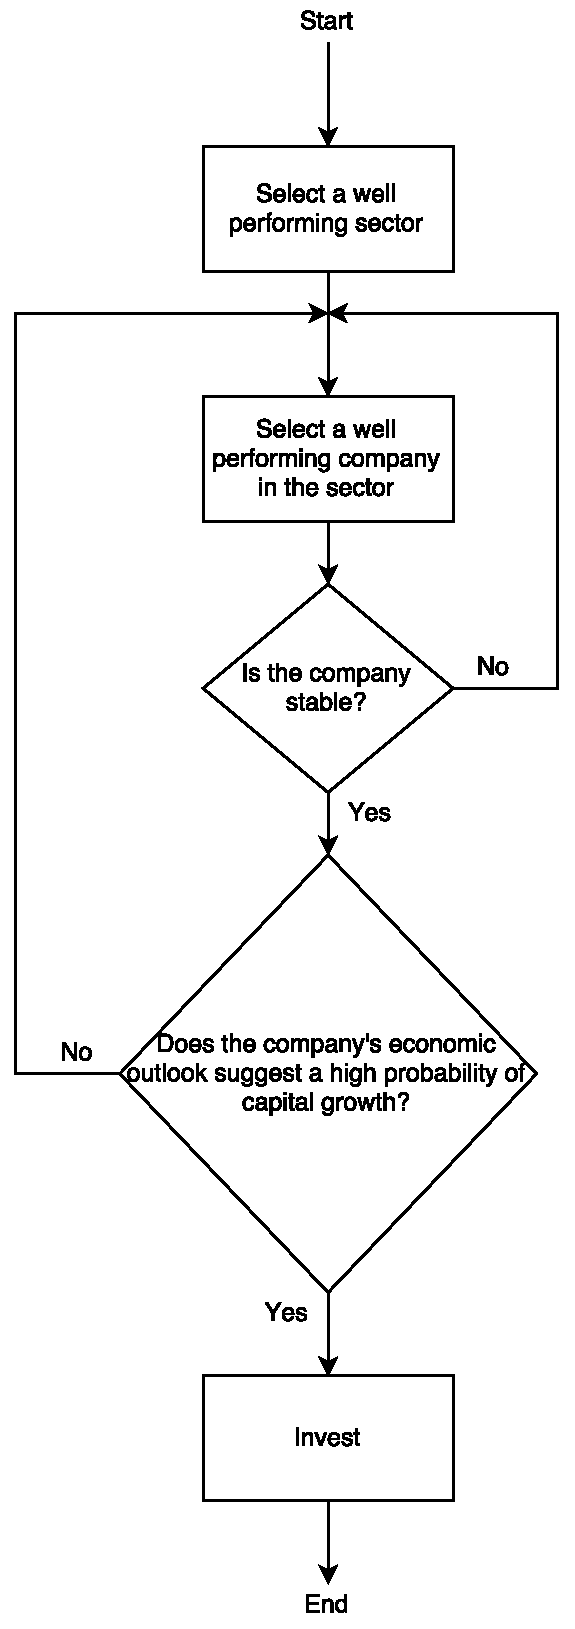
\includegraphics[scale=0.5]{decisions.pdf}
\caption{Flow diagram of investment selection}
\label{fig:flowChart}
\end{figure}

\label{sec:flowChart}



\bibliographystyle{plain}
\bibliography{bib} 



\end{document}
